\section{1174083 - Bakti Qilan Mufid}
Chapter 9 - Conditional Generative Adversarial Network
\subsection{Teori}
\subsubsection{Jelaskan dengan ilustrasi gambar sendiri apa perbedaan antara vanilla GAN dan cGAN.}
\hfill\\
\begin{enumerate}
\item Vanilla GAN merupakan tipe paling sederhana dari tipe-tipe yang ada pada GAN. Generator dan diskriminator adalah perceptron multi-layer sederhana. Perceptron adalah salah satu metode Jaringan Syaraf Tiruan (JST) sederhana yang menggunakan algoritma training untuk melakukan klasifikasi secara linier. Perceptron digunakan untuk melakukan klasifikasi sederhana dan membagi data untuk menentukan data mana yang masuk dalam klasifikasi dan data mana yang missclasifikasi (diluar klasifikasi). Vanilla GAN mengoptimalkan persamaan matematika menggunakan keturunan gradien stokastik(mempunyai unsur peluang).

\item cGAN(conditional GAN) merupakan tipe GAN yang dikondisikan pada beberapa tambahan informasi. Dalam GAN-projects informasi tambahan itu adalah y yang dimasukan ke generator sebagai lapisan input tambahan.

berikut gambaran antara Vanilla GAN dan cGAN 
\end{enumerate}
\begin{figure}[H]
	\centering
	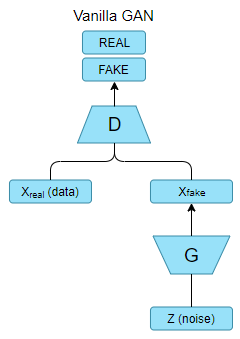
\includegraphics[width=4cm]{figures/1174083/figures9/1.png}
	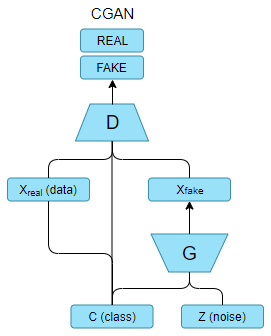
\includegraphics[width=4cm]{figures/1174083/figures9/1a.png}
	\caption{gambaran penjelasan no. 1}
\end{figure}

\subsubsection{Jelaskan dengan ilustrasi gambar sendiri arsitektur dari Age-cGAN.}
\hfill\\
Age-cGAN terdiri dari empat jaringan, yaitu:
\begin{itemize}
\item Encoder, pemetaan terbalik dari gambar wajah input dan usia kondisi dengan vektor laten.
\item FaceNet(face recognition network), mempelajari perbedaan antara gambar input x dan sebuah gambar yang direkonstruksi. 
\item Generator, membutuhkan sebuah representasi tersembunyi yang terdiri dari gambar wajah dan kondisi vektor  dan  akan menghasilkan gambar.
\item Discriminator, melakukan diskriminasi antara gambar asli dan gambar palsu.
\end{itemize}

\begin{figure}[H]
	\centering
	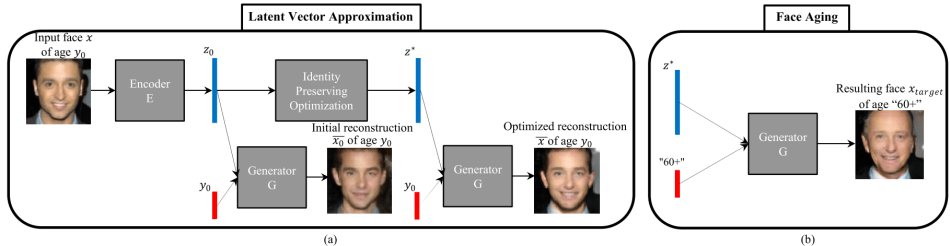
\includegraphics[width=10cm]{figures/1174083/figures9/2.png}
	\caption{gambaran penjelasan no. 2}
\end{figure}

\subsubsection{Jelaskan dengan ilustrasi gambar sendiri arsitektur encoder network dari Age-cGAN.}
\hfill\\
Tujuan utama dari encoder network adalah menghasilkan latent vector dari gambar yang sudah disediakan. Pada dasarnya, dibutuhkan gambar dengan dimensi (64, 64, 3) lalu akan diubah mejadi vektor 100-dimensi.encoder network juga merupakan deep CNN. encoder network berisi empat blok konvolusional dan dua dense layer. pada setiap blok konvolusional mengandung sebuah layer konvolusional, batch normalization, dan fungsi aktivasi. Di setiap blok konvolusional, setiap konvolusional lapisan diikuti oleh lapisan normalisasi batch, kecuali yang pertama.
\begin{figure}[H]
	\centering
	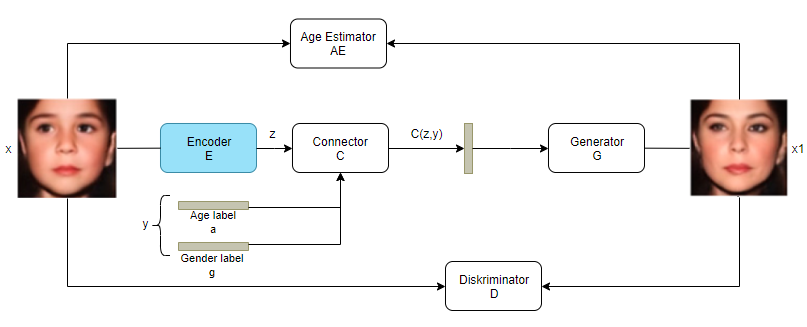
\includegraphics[width=10cm]{figures/1174083/figures9/3.png}
	\caption{gambaran penjelasan no. 3}
\end{figure}


\subsubsection{Jelaskan dengan ilustrasi gambar sendiri arsitektur generator network dari Age-cGAN.}
\hfill\\
Tujuan utama dari generator network adalah menghasilkan gambar dengan dimensi (64,64,3). dibutuh kan vektor 100-dimensi dan beberapa tambahan informasi, y, dan mencoba menghasilkan gambar yang realistis. generator juga merupakan deep CNN, yang terbuat dari layer dense, upsampling, dan konvolusional layer. Dibutuhkan dua nilai input: sebuah noise vektor dan conditional value. Conditional value adalah informasi tambahan yang diberikan generator network. Untuk Age-cGAN, informasi tersebut merupakan usia.

\begin{figure}[H]
	\centering
	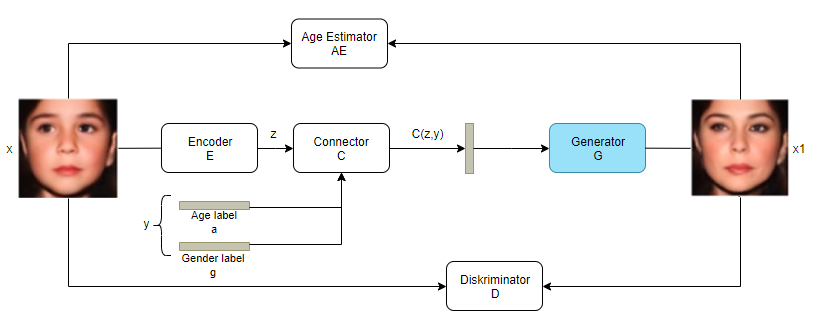
\includegraphics[width=10cm]{figures/1174083/figures9/4.png}
	\caption{gambaran penjelasan no. 4}
\end{figure}

\subsubsection{Jelaskan dengan ilustrasi gambar sendiri arsitektur discriminator network dari Age-cGAN.}
\hfill\\
Tujuan utama dari diskriminator network adalah untuk mengidentifikasi apakah gambar itu asli atau palsu, yang diketahui dengan cara mengolah gambar dalam downsampling dan beberapa lapisan classification. atau bisa disebut memprediksi gambar tersebut palsu atau asli. diksriminator network juga merupakan deep CNN. diskriminator network juga terdiri dari beberapa konvolusional blok. setiap konvolusional blok memiliki konvolusional layer, kumpulan normalisasi layer, dan fungsi aktivasi. kecuali konvolusional blok pertama yang tidak memiliki kumpulan normalisasi layer.

\begin{figure}[H]
	\centering
	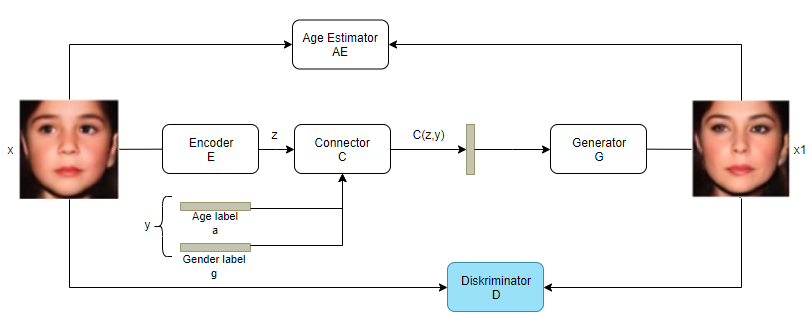
\includegraphics[width=10cm]{figures/1174083/figures9/5.png}
	\caption{gambaran penjelasan no. 5}
\end{figure}

\subsubsection{Jelaskan dengan ilustrasi gambar apa itu pretrained Inception-ResNet-2 Model.}
\hfill\\
Inception-ResNet-2 adalah jaringan saraf konvolusional(CNN) yang dilatih oleh lebih dari satu juta gambar dari database ImageNet(http://www.image-net.org). Jaringanya memiliki 164 lapisan dan dapat mengklasifikasikan gambar kedalam 1000 kategori objek, seperti keyboard, mouse, pensil, dan maca-macam binatang. hasilnya, jaringan tersebut sudah mempelajari representasi fitur yang kaya untuk berbagai gambar. jaraingan ini memiliki ukuran input gambar 299-by-299.

\begin{figure}[H]
	\centering
	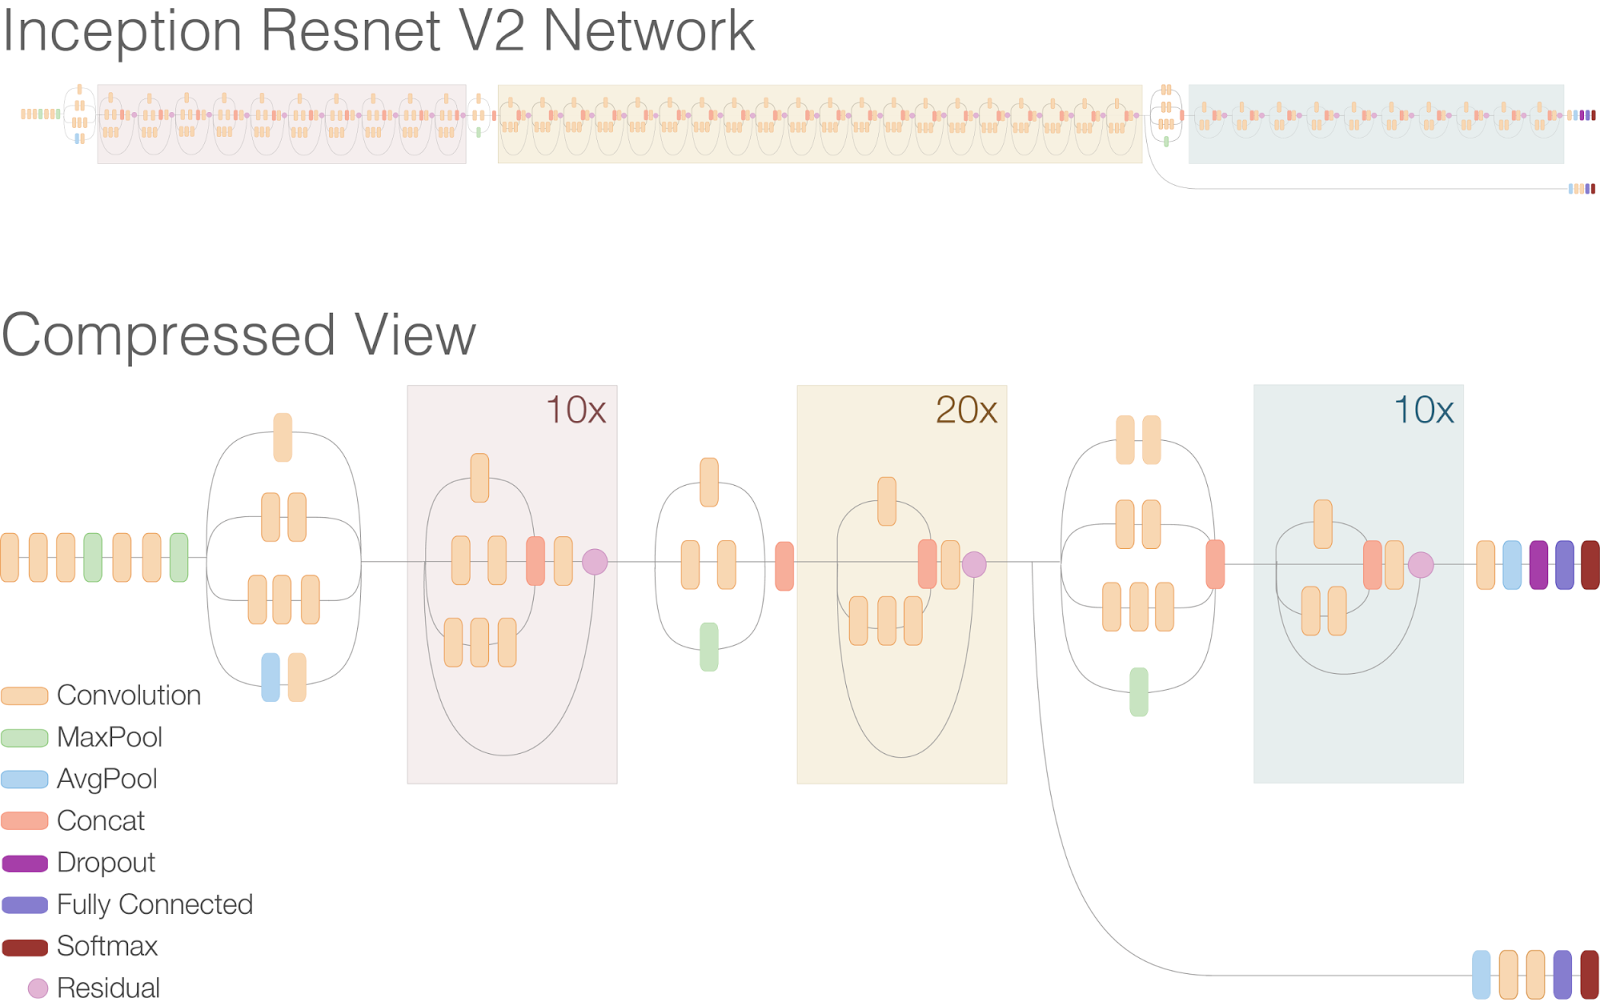
\includegraphics[width=12cm]{figures/1174083/figures9/6.png}
	\caption{gambaran penjelasan no. 6}
\end{figure}

\subsubsection{Jelaskan dengan ilustrasi gambar sendiri arsitektur Face recognition network Age-cGAN.}
\hfill\\
Tujuan utama dari Face recognition adalah untuk mengenali identitas seseorang dalam gambar yang diberikan.

\begin{figure}[H]
	\centering
	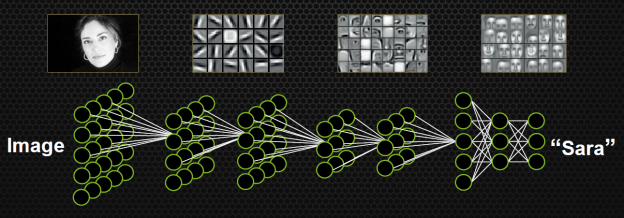
\includegraphics[width=10cm]{figures/1174083/figures9/7.png}
	\caption{gambaran penjelasan no. 7}
\end{figure}

\subsubsection{Sebutkan dan jelaskan serta di sertai contoh-contoh tahapan dari Age-cGAN}
\hfill\\
tahapan dari Age-cGAN ada tiga tahap, diantaranya:
\begin{enumerate}
\item Conditional GAN training, pada tahap ini Age-cGAN melatih generator dan diskriminator network.
\item Initial latent vector approximation, pada tahap ini Age-cGAN melatih encoder network.
\item Latent vector optimization, pada tahap ini Age-cGAN mengoptimalkan encoder dan generator network.
\end{enumerate}

\begin{figure}[H]
	\centering
	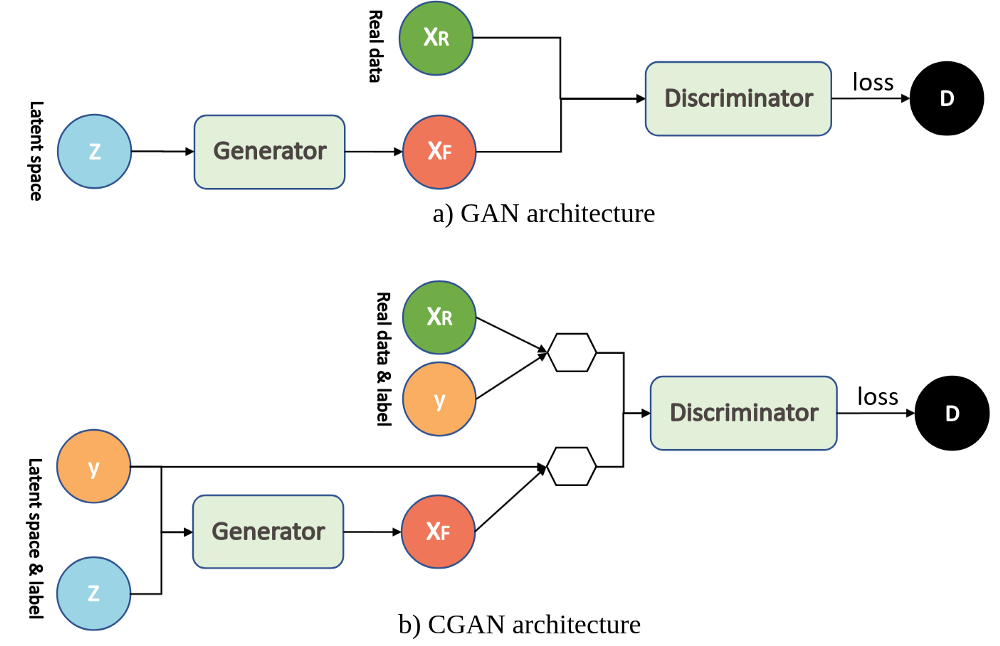
\includegraphics[width=10cm]{figures/1174083/figures9/8.png}
	\caption{gambaran penjelasan no. 8(Conditional GAN training)}
\end{figure}
\begin{figure}[H]
	\centering
	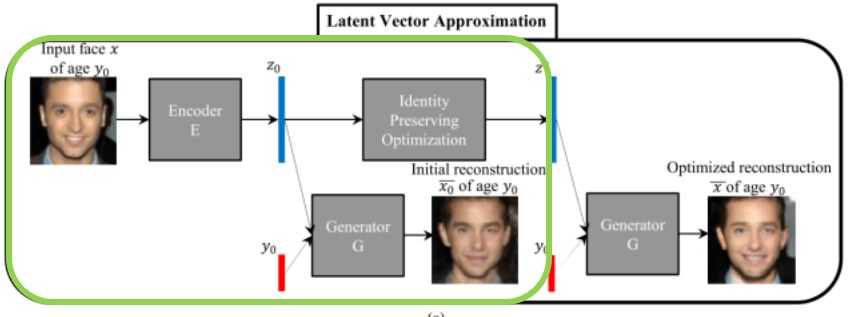
\includegraphics[width=10cm]{figures/1174083/figures9/8a.png}
	\caption{gambaran penjelasan no. 8(Initial latent vector approximation)}
\end{figure}
\begin{figure}[H]
	\centering
	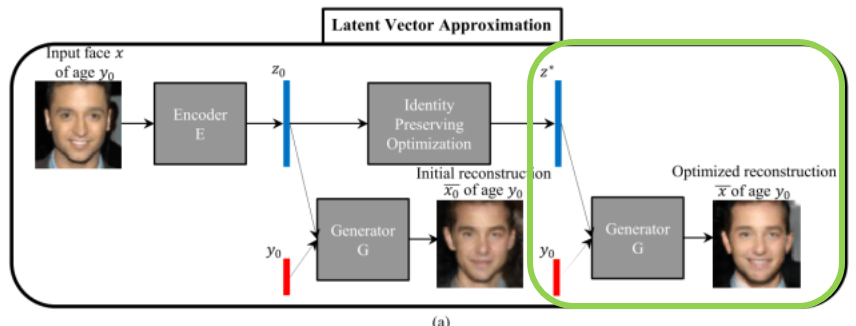
\includegraphics[width=10cm]{figures/1174083/figures9/8b.png}
	\caption{gambaran penjelasan no. 8(Latent vector optimization)}
\end{figure}

\subsubsection{Berikan contoh perhitungan fungsi training objektif}
\hfill\\
melatih jaringan cGAN melibatkan optimalisasi fungsi $\nu(\Theta _{G},\Theta _{D})$. melatih cGAN bisa dianggap game minimax(Algoritma minimax akan melakukan pengecekan pada seluruh kemungkinan yang ada, sehingga akan menghasilkan pohon permainan yang berisi semua kemungkinan permainan tersebut), dimana generator dan diskriminator keduanya dilatih secara bersamaan. Dalam persamaan sebelumnya $P_{x}$ merupakan parameter jaringan generator, $\Theta _{D}$ merupakan parameter G dan D, $logD(x,y)$ merupaka loss dari model diskriminator, $log(1-D(G(z,\tilde{y}),\tilde{y}))$ merupakan loss dari model generator, dan $P_{data}$ merupakan distribusi dari kemungkinan semua gambar.
\begin{figure}[H]
	\centering
	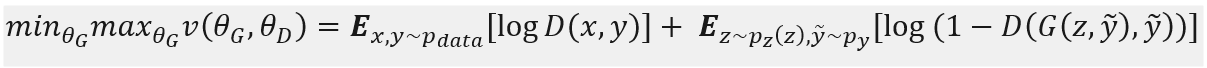
\includegraphics[width=10cm]{figures/1174083/figures9/9.png}
	\caption{gambaran penjelasan no. 9}
\end{figure}

\subsubsection{Berikan contoh dengan ilustrasi penjelasan dari Initial latent vector approximation}
\hfill\\
Perkiraan latent vektor awal adalah metode yang memperkirakan latent vektor untuk mengoptimalkan rekontruksi gambar wajah. untuk itu maka diperlukan network encoder. network encoder dilatih oleh gambar yang digenerate dan gambar yang nyata. setelah dilatih, network encoder akan mulai menghasilkan vektor laten dari distribusi yang dipelajari. fungsiya untuk melatih network encoder sebagai Euclidean distence loss.
\begin{figure}[H]
	\centering
	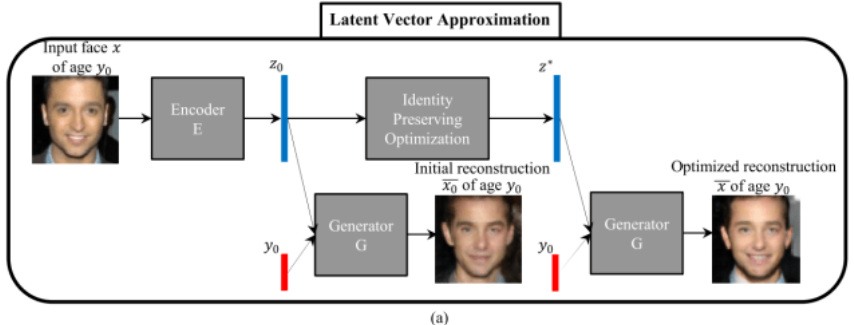
\includegraphics[width=10cm]{figures/1174083/figures9/10.png}
	\caption{gambaran penjelasan no. 10}
\end{figure}


\subsubsection{Berikan contoh perhitungan latent vector optimization}
\hfill\\
ketika latent vector optimization berlangsung, Age-cGAN mengoptimalkan network encoder dan network generator secara bersamaan. persamaan yang akan digunakan adalah seperti berikut:
\[z*IP = argmin_{z}||FR(x)- FR(\bar{x})||L_{2}\]

$FR$ adalah jaringan pengenalan wajah. persamaan ini menunjukan bahwa jarak Euclidean antara gambar asli dan gambar yang direkontruksi harus minimal. pada tahap ini, Age-cGAN mencoba meminimalkan jarak dan memaksimalkan pelestarian identitas.

\subsection{Praktek}
\subsubsection{Jelaskan bagaimana cara ekstrak file dataset Age-cGAN menggunakan google colab}
\hfill\\
Caranya cukup mudah, kita tinggal iktui langkah-langkah berikut:
\begin{itemize}
\item Login terlebih dahulu ke google colab menggunakan akun google
\item lalu buka link datasetnya (https://drive.google.com/open?id=1NoV357ZvemE5dLCGySNTo6YNXsU8LyUs) lalu copy dataset ke akun google drive.
\item Setelah di copy, buka google colab, buat notebook baru dan klik Mount Drive
\item Lalu unzip file wiki\_crop.tar. maka dataset siap digunakan. 
\end{itemize}
\begin{figure}[H]
	\centering
	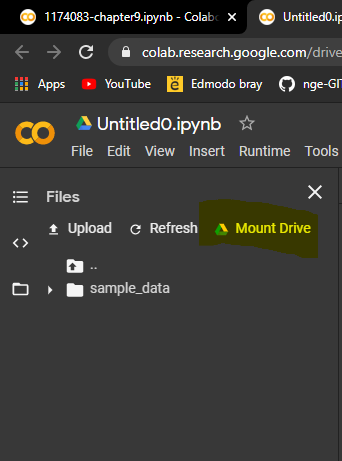
\includegraphics[scale=0.5]{figures/1174083/figures9/p1.png}
	\caption{gambar penjelasan praktek soal no.1}
\end{figure}

\subsubsection{Jelaskan bagaimana kode program bekerja untuk melakukan load terhadap dataset yang sudah di ekstrak, termasuk bagaimana penjelasan kode program perhitungan usia}
\hfill\\
file dataset wiki\_crop.tar berisi 62.328 gambar dan sebuah file bernama wiki.mat yang menampung labelnya. Library spicy.io mempunyai method yang bernama loadmat, dimana method tersebut sangat memudahkan ketika kita ingin me-load file .mat. lalu untuk me-load datanya, kita bisa menggunakan kode berikut:
\lstinputlisting[firstline=195, lastline=219]{src/1174083/src9/run.py}

variabel photo\_taken adalah daftar tahun dan dob adalah tanggal serial Matlab nomor untuk gambar yang sesuai dalam daftar. kita bisa mengukur umur seseorang dari seri tanggal dan tahun gambar tersebut diambil, dengan menggunakan kode berikut:
\lstinputlisting[firstline=186, lastline=192]{src/1174083/src9/run.py}

\subsubsection{Jelaskan bagaimana kode program The Encoder Network bekerja dijelaskan dengan bahasa awam dengan ilustrasi sederhana}
\hfill\\
Berikut merupakan langkah-langkah encoder network bekerja:
\begin{enumerate}
\item Mulai dengan membuat layer input
\lstinputlisting[firstline=22, lastline=22]{src/1174083/src9/run.py}

\item Lalu tambahkan blok konvolusi pertama, yang berisi lapisan konvolusi 2D dan fungsi aktivasi dengan konfigurasi sebagai berikut:
	\begin{itemize}
		\item Filters: 32
		\item Kernel size: 5
		\item Strides: 2
		\item Padding: same
		\item Activation: LeakyReLU with alpha equal to 0.2:
	\end{itemize}
\lstinputlisting[firstline=24, lastline=27]{src/1174083/src9/run.py}

\item Selanjutnya, tambahkan tiga blok konvolusi lagi, yang masing-msaing berisi lapisan konvolusi 2D dan diikuti oleh lapisan normalisasi batch serta fungsi aktivasi, seperti pada konfigurasi berikut:
	\begin{itemize}
		\item Filters: 64, 128, 256
		\item Kernel size: 5, 5, 5
		\item Strides: 2, 2, 2
		\item Padding: same, same, same
		\item Batch normalization: Each convolutional layer is followed by a batch
		\item normalization layer
		\item Activations: LealyReLU, LeakyReLU, LeakyReLU with alpha equal to 0.2:
	\end{itemize}
\lstinputlisting[firstline=29, lastline=42]{src/1174083/src9/run.py}

\item Selanjutnya meratakan(flatten) output dari blok konvolusi yang terakhir, sebagai berikut:
\lstinputlisting[firstline=44, lastline=45]{src/1174083/src9/run.py}

\item Selanjutnya tambahkan dense layer(yang terhubung secara penuh) dan dikikuti dengan batch normaisasi layer serta fungsi aktivasi, dengan konfigurasi berikut:
	\begin{itemize}
		\item Units (nodes): 2,096
		\item Batch normalization: Yes
		\item Activation: LeakyReLU with alpha equal to 0.2:
	\end{itemize}
\lstinputlisting[firstline=47, lastline=50]{src/1174083/src9/run.py}

\item Selanjutnya, tambahkan dense layer kedua(yang terhubung secara penuh), dengan konfigurasi berikut:
	\begin{itemize}
		\item Units (nodes): 100
		\item Activation: None:
	\end{itemize}
\lstinputlisting[firstline=52, lastline=53]{src/1174083/src9/run.py}
	
\item Terakhir, buat model Keras dan tentukan input serta output untuk network encoder.
\lstinputlisting[firstline=56, lastline=56]{src/1174083/src9/run.py}
\end{enumerate}

\subsubsection{Jelaskan bagaimana kode program The Generator Network bekerja dijelaskan dengan bahasa awam dengan ilustrasi sederhana}
\hfill\\
Berikut merupakan langkah-langkah generator network bekerja:
\begin{enumerate}
\item Mulai dengan membuat dua lapisan input ke generator network.
\lstinputlisting[firstline=64, lastline=68]{src/1174083/src9/run.py}

\item Selanjutnya, gabungkan input sepanjang dimensi channel, seperti berikut:
\lstinputlisting[firstline=70, lastline=70]{src/1174083/src9/run.py}	

\item Lalu tambahkan blok dense (terhubung secara penuh) dengan konfigurasi berikut:
	\begin{itemize}
		\item Units (nodes): 2,048
		\item Input dimension: 106
		\item Activation: LeakyReLU with alpha equal to 0.2
		\item Dropout: 0.2:
	\end{itemize}
\lstinputlisting[firstline=72, lastline=74]{src/1174083/src9/run.py}	

\item Selanjutnya tambahkan blok dense kedua, dengan konfigurasi berikut:
	\begin{itemize}
		\item Units (nodes): 16,384
		\item Batch normalization: Yes
		\item Activation: LeakyReLU with alpha equal to 0.2
		\item Dropout: 0.2:	
	\end{itemize}
\lstinputlisting[firstline=76, lastline=79]{src/1174083/src9/run.py}	

\item Selanjutnya bentuk kembali output dari lapisan dense terakhir ke 3D tensor dengan dimensi(8,8,256):
\lstinputlisting[firstline=81, lastline=81]{src/1174083/src9/run.py}	

\item Selanjutnya tambahkan blok upsampling yang berisi lapisan upsampling diikuti oleh lapisan konvolusi 2D serta batch normalisasi dengan konfigurasi berikut:
	\begin{itemize}
		\item Upsampling size: (2, 2)
		\item Filters: 128
		\item Kernel size: 5
		\item Padding: same
		\item Batch normalization: Yes, with momentum equal to 0.8
		\item Activation: LeakyReLU with alpha equal to 0.2:
	\end{itemize}
\lstinputlisting[firstline=83, lastline=86]{src/1174083/src9/run.py}	

\item Selanjutnya, tambahkan blok upsampling lain(mirip dengan lapisan sebelumnya), seperti pada kode berikut, dan konfigurasinya mirip seperti blok sebelumnya, kecuali jumlah filter yang digunakan dalam lapisan konvolusi yang asalnya 128 menjadi 64:
\lstinputlisting[firstline=81, lastline=91]{src/1174083/src9/run.py}	

\item Selanjutnya tambahkan blok upsampling terkahir. konfigurasinya mirip dengan lapisan sebelumnya, kecuali tiga lapisan filter akan digunakan dan batch normalisasi tidak digunakan:
\lstinputlisting[firstline=93, lastline=95]{src/1174083/src9/run.py}

\item Terakhir, buat model Keras dan tentukan input serta output untuk generator network:
\lstinputlisting[firstline=97, lastline=97]{src/1174083/src9/run.py}

\end{enumerate}

\subsubsection{Jelaskan bagaimana kode program The Discriminator Network bekerja dijelaskan dengan bahasa awam dengan ilustrasi sederhana}
\hfill\\
Berikut merupakan langkah-langkah diskriminator network bekerja:
\begin{enumerate}
\item Mulailah dengan membuat dua lapisan input, karena pada project ini dikriminator akan memproses dua input:
\lstinputlisting[firstline=112, lastline=115]{src/1174083/src9/run.py}

\item Selanjutnya, tambahkan blok konvolusi 2D (fungsi Conv2D + aktivasi) dengan konfigurasi berikut:
	\begin{itemize}
		\item Filters = 64
		\item Kernel size: 3
		\item Strides: 2
		\item Padding: same
		\item Activation: LeakyReLU with alpha equal to 0.2:
	\end{itemize}
\lstinputlisting[firstline=117, lastline=118]{src/1174083/src9/run.py}

\item Selanjutnya perluas label\_input sehingga memiliki bentuk (32,32,6):
\lstinputlisting[firstline=120, lastline=120]{src/1174083/src9/run.py}
fungsi expand\_label\_input sebgai berikut:
\lstinputlisting[firstline=101, lastline=105]{src/1174083/src9/run.py}

\item Selanjutnya gabungkan tensor label yang telah ditransformasi dan output terakhir dari lapisan konvolusi, seperti berikut: 
\lstinputlisting[firstline=121, lastline=121]{src/1174083/src9/run.py}

\item Tambahkan blok konvolusi (lapisan konvolusi 2D + batch normalisasi + fungsi aktivasi) dengan konfigurasi berikut:
	\begin{itemize}
		\item Filters: 128
		\item Kernel size: 3
		\item Strides: 2
		\item Padding: same
		\item Batch normalization: Yes
		\item Activation: LeakyReLU with alpha equal to 0.2:
	\end{itemize}
\lstinputlisting[firstline=123, lastline=125]{src/1174083/src9/run.py}

\item Selanjutnya tambahkan dua blok konvolusi lagi, seperti berikut:
\lstinputlisting[firstline=127, lastline=133]{src/1174083/src9/run.py}

\item Lalu tambahkan lapisan flatten
\lstinputlisting[firstline=135, lastline=135]{src/1174083/src9/run.py}

\item lalu tamabahkan lapisan dense(lapisan pengklasifikasian) yang menghasilkan probabilitas:
\lstinputlisting[firstline=136, lastline=136]{src/1174083/src9/run.py}

\item Terakhir, buat model Keran dan tentukan input serta output untuk diskriminator network.
\lstinputlisting[firstline=138, lastline=138]{src/1174083/src9/run.py}

\end{enumerate}

\subsubsection{Jelaskan bagaimana kode program Training cGAN bekerja dijelaskan dengan bahasa awam dengan ilustrasi sederhana}
\hfill\\
Berikut adalah langkah-langkah melatih cGAN:
\begin{enumerate}
\item Mulailah dengan menentukan parameter yang diperlukan untuk pelatihan:
\lstinputlisting[firstline=305, lastline=315]{src/1174083/src9/run.py}

\item Selanjutnya, tentukan optimisator untuk pelatihan. Kali ini kita akan menggunakan Adam optimizer yang terdapat di Keras. untuk inisiasinya seperti berikut
\lstinputlisting[firstline=317, lastline=323]{src/1174083/src9/run.py}
gunakan equal rate sama dengan 0,0002, nilai beta\_1 sama dengan 0,5, nilai beta\_2 sama dengan 0,999, dan nilai epsilon sama dengan 10e-8 semua optimizer.

\item Selanjutnya, muat dan kompilasi generator network dan diskriminator network. Dalam Keras kita harus mengkompilasi network terlebih dahulu sebelum melatihnya.
\lstinputlisting[firstline=328, lastline=334]{src/1174083/src9/run.py}

\item Selanjutnya, buat dan kompilasi model adversial, sebagai berikut:
\lstinputlisting[firstline=336, lastline=343]{src/1174083/src9/run.py}

\item Selanjutnya tambahkan TensorBoard untuk menyimpan losses, se[erti berikut:
\lstinputlisting[firstline=345, lastline=347]{src/1174083/src9/run.py}

\item Selanjutnya load semua gambar menggunakan fungsi load\_data yang didefinisikan pada bagian mempersiapkan data:
\lstinputlisting[firstline=352, lastline=352]{src/1174083/src9/run.py}

\item Selanjutnya konversikan nilai numerik usia ke kategori usia, seperti berikut:
\lstinputlisting[firstline=353, lastline=353]{src/1174083/src9/run.py}
Definisi dari fungsi age\_to\_category seperti kode berikut:
\lstinputlisting[firstline=222, lastline=241]{src/1174083/src9/run.py}

\item Selanjutnya load semua gambar dan buat ndarray yang berisi semua gambar:
\lstinputlisting[firstline=359, lastline=360]{src/1174083/src9/run.py}
Definisi dari fungsi load\_data seperti kode berikut:
\lstinputlisting[firstline=244, lastline=267]{src/1174083/src9/run.py}

\item Selanjutnya buat perulangan(for) berdasarkan jumlah epoch, seperti berikut:
\lstinputlisting[firstline=370, lastline=377]{src/1174083/src9/run.py}

\item Selanjutnya buat perulangan yang lain didalam perulangan epoch berdasarkan num\_batches, seperti berikut:
\lstinputlisting[firstline=378, lastline=379]{src/1174083/src9/run.py}

\item Selanjutnya buat sample dari batch gambar dari dataset yang asle dan batch dari one-hot encoded age vector:
\lstinputlisting[firstline=381, lastline=385]{src/1174083/src9/run.py}
bentuk dari image\_batch (batch\_size, 64, 64, 3) dan bentuk dari y\_batch (batch\_size, 6).

\item Selanjutnya buat sampel batch noise vektor dari distribusi Gaussian, seperti berikut:
\lstinputlisting[firstline=386, lastline=386]{src/1174083/src9/run.py}

\item Selanjutnya buat gambar palsu(fake) menggunakan generator network. perlu diingat bahwa kita belum melatih network generator.
\lstinputlisting[firstline=392, lastline=393]{src/1174083/src9/run.py}

\item Sekarang latih network diskriminator pada gambar yang asli dan juga gambar yang palsu
\lstinputlisting[firstline=395, lastline=396]{src/1174083/src9/run.py}

\item Lalu latih adversial network dan mempause diskriminator network. atau kita hanya akan melatih generator network.
\lstinputlisting[firstline=404, lastline=411]{src/1174083/src9/run.py}

\item Selanjutnya hitung dan cetak lossesnya:
\lstinputlisting[firstline=413, lastline=416]{src/1174083/src9/run.py}

\item Selanjutnya tulis losses ke TensorBoard untuk divisualisasikan  
\lstinputlisting[firstline=418, lastline=420]{src/1174083/src9/run.py}

\item Buat sampel dan simpan gambar setiap 10 epoch, seperti berikut:
\lstinputlisting[firstline=425, lastline=436]{src/1174083/src9/run.py}
Letakan blok kode sebelumnya didalan perulangan epoch. setelah setiap 10 epoch, maka akan menghasilkan batch dari gambar palsu dan akan disimpan ke direktori results. untuk fungsi save\_rgb\_img adalah sebagai fungsi utilitas dan didefinisikan se[erti berikut:
\lstinputlisting[firstline=290, lastline=301]{src/1174083/src9/run.py}

\item Terakhir simpan kedua model dengan menambahkan baris berikut:
\lstinputlisting[firstline=580, lastline=582]{src/1174083/src9/run.py}

\end{enumerate}

\subsubsection{Jelaskan bagaimana kode program Initial dan latent vector approximation bekerja dijelaskan dengan bahasa awam dengan ilustrasi sederhana}
\hfill\\
Seperti yang sudah diketahui bahawa cGAN tidak belajar untuk memetakan balik dari gambar ke vektor latent. oleh karena itu, encoder yang akan mempelajari pemetaan balik ini dan mampu menghasilkan vektor laten yang dapat digunakan untuk menghasilkan gambar wajah pada usia yang ditargetkan. 

Kita telah mendefinisikan hyperparameter yang dibutuhkan dalam pelatihan. Dan untuk langkah-langkahnya seperti berikut:

\begin{enumerate}
\item Mulailah dengan membuat network encoder. tambahkan kode berikut untuk membuat dan mengkompilasi network encoder.
\lstinputlisting[firstline=450, lastline=452]{src/1174083/src9/run.py}
Jika belum mendefinisikan euclidean\_distence\_loss, maka definisikan terlebih dahulu seperti pada kode berikut:
\lstinputlisting[firstline=584, lastline=588]{src/1174083/src9/run.py}

\item Selanjutnya load network generator, seperti berikut:
\lstinputlisting[firstline=456, lastline=456]{src/1174083/src9/run.py}

\item Selanjutnya buat sampel batc vektor latent, seprti berikut:
\lstinputlisting[firstline=460, lastline=460]{src/1174083/src9/run.py}

\item Selanjutnya buat sampel batch acak angka usia dan konversikan usia angka acak tadi kedalam one-hot encoded vector, seperti berikut:
\lstinputlisting[firstline=462, lastline=465]{src/1174083/src9/run.py}

\item Selanjutnya tambahkan perulangan epoch dan batch dari langkha-langkah. seperti berikut:
\lstinputlisting[firstline=467, lastline=475]{src/1174083/src9/run.py}

\item Sekarang buat sampel batch vektor latent dan batch one-hot encoded vector dari 1000 sampel, seperti berikut:
\lstinputlisting[firstline=477, lastline=478]{src/1174083/src9/run.py}

\item Selanjutnya hasilkan gambar palsu menggunakan network generator yang sudah dilatih:
\lstinputlisting[firstline=480, lastline=480]{src/1174083/src9/run.py}

\item Lalu latih network encoder pada gambar yang dihasilkan oleh network generator:
\lstinputlisting[firstline=482, lastline=483]{src/1174083/src9/run.py}

\item Selanjutnya tulis loss encoder ke TensorBoard pada setiap epoch.
\lstinputlisting[firstline=488, lastline=489]{src/1174083/src9/run.py}

\item dan kita perlu menyimpan network encoder yang sudah dilatih. simpan model encoder dengan kode berikut:
\lstinputlisting[firstline=491, lastline=492]{src/1174083/src9/run.py}
\end{enumerate}

\subsection{Penanganan Error}
\subsubsection{Terjadi error}
\hfill\\
%\begin{enumerate}
%\item terjadi error Summary has no attribute, seperti pada gambar berikut:
%\begin{figure}[H]
%	\centering
%	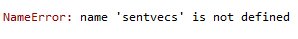
\includegraphics[scale=0.5]{figures/1174083/figures9/error1.png}
%	\caption{terjadi Error 1}
%\end{figure}
%\end{enumerate}

\subsubsection{Solusi}
\hfill\\
%\begin{enumerate}
%\item solusi dari error 1 ialah:
%dengan menginstall versi tensorflow 1.xx
%\begin{figure}[H]
%	\centering
%	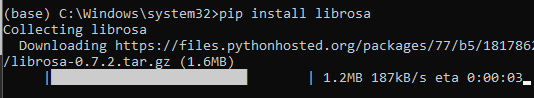
\includegraphics[scale=0.5]{figures/1174083/figures9/s1.png}
%	\caption{solusi Error 1}
%\end{figure}
%\end{enumerate}

\subsection{Bukti Tidak Plagiat}
\begin{figure}[H]
	\centering
	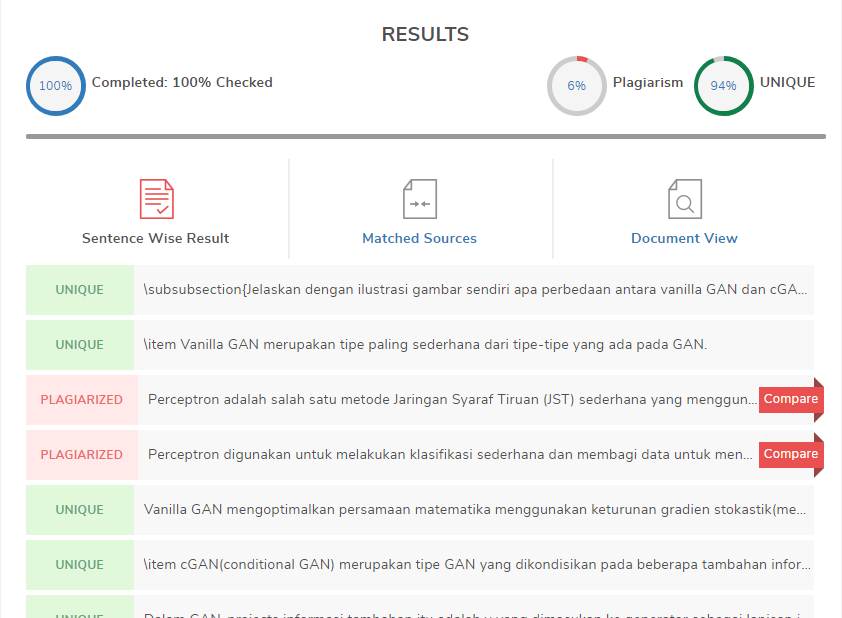
\includegraphics[width=12cm]{figures/1174083/figures9/plagiarisme1.png}
	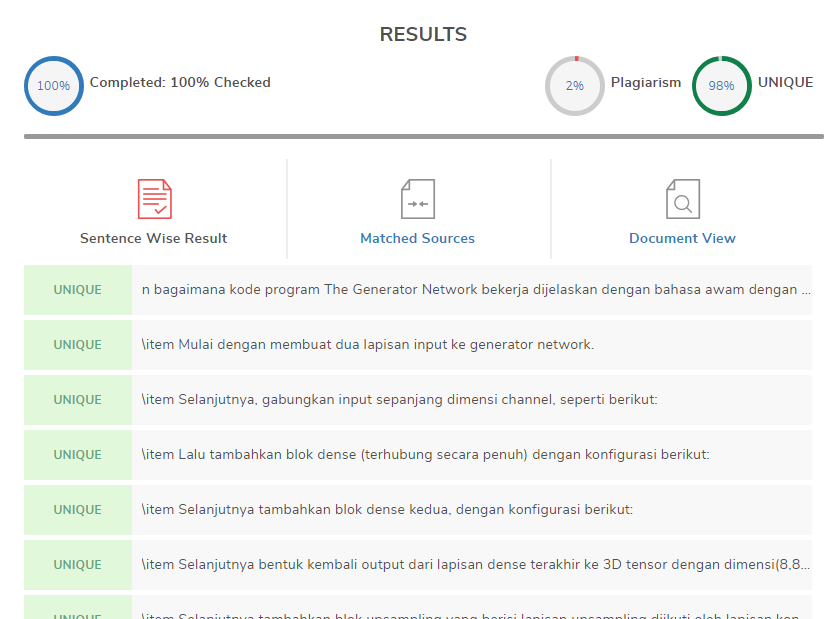
\includegraphics[width=12cm]{figures/1174083/figures9/plagiarisme2.png}
	\caption{Bukti tidak plagiat}
\end{figure}

\subsection{Link Youtube}
https://bit.ly/baktiListVideo